%%%%%%%%%%%%%%%%%%%%%%%%%%%%%%%%%%%%%%%%%%%%%%%%%%%%%%%%%%%%%%%
% Welcome to the MAT320 Homework template on Overleaf -- just edit your
% LaTeX on the left, and we'll compile it for you on the right.
%%%%%%%%%%%%%%%%%%%%%%%%%%%%%%%%%%%%%%%%%%%%%%%%%%%%%%%%%%%%%%%
% --------------------------------------------------------------
% Based on a homework template by Dana Ernst.
% --------------------------------------------------------------
% This is all preamble stuff that you don't have to worry about.
% Head down to where it says "Start here"
% --------------------------------------------------------------

\documentclass[12pt]{article}

\usepackage{graphicx}
\graphicspath{{./images/}}
\usepackage{textcomp} % cent symbol, such as \textcent
\usepackage[margin=1in]{geometry} 
\usepackage{amsmath,amsthm,amssymb}
\usepackage{cancel}
\usepackage{mathtools} % ceiling function
\DeclarePairedDelimiter{\ceil}{\lceil}{\rceil}
% https://tex.stackexchange.com/questions/146306/how-to-make-horizontal-lists
\usepackage[inline]{enumitem} % allows using letters in enumerate list environment

% source: https://stackoverflow.com/questions/3175105/inserting-code-in-this-latex-document-with-indentation

\usepackage{listings}
\usepackage{color}

\definecolor{dkgreen}{rgb}{0,0.6,0}
\definecolor{gray}{rgb}{0.5,0.5,0.5}
\definecolor{mauve}{rgb}{0.58,0,0.82}

\lstset{frame=tb,
	language=C, % language for code listing
	aboveskip=3mm,
	belowskip=3mm,
	showstringspaces=false,
	columns=flexible,
	basicstyle={\small\ttfamily},
	numbers=none,
	numberstyle=\tiny\color{gray},
	keywordstyle=\color{blue},
	commentstyle=\color{dkgreen},
	stringstyle=\color{mauve},
	breaklines=true,
	breakatwhitespace=true,
	tabsize=4
}

\newcommand{\N}{\mathbb{N}}
\newcommand{\Z}{\mathbb{Z}}

\newenvironment{ex}[2][Exercise]{\begin{trivlist}
		\item[\hskip \labelsep {\bfseries #1}\hskip \labelsep {\bfseries #2.}]}{\end{trivlist}}

\newenvironment{sol}[1][Solution]{\begin{trivlist}
		\item[\hskip \labelsep {\bfseries #1:}]}{\end{trivlist}}


\begin{document}

% --------------------------------------------------------------
%                         Start here
% --------------------------------------------------------------

\noindent Sergio Garcia Tapia \hfill

\noindent{\small Computer Systems: A Programmer's Perspective, by Bryant and O'Hallaron} \hfill

\noindent{\small Chapter 12: Concurrent Programming}

\noindent\today

\subsection*{Practice Problems}

\begin{ex}{12.1}
	After the parent closes the connected descriptor in line 33 of the concurrent server in
	Figure~12.5, the child is still able to communicate with the client using its copy of the
	descriptor. Why?
\end{ex}

\begin{sol}
	\
	When the parent forks a child to handle the request for the client, an identical but independent
	file descriptor table is created for it. The file descriptors reference the same entries in
	the table of open descriptions (file). As a result, the reference count of each connected
	descriptor that existed before the fork increases to 2. The call to \texttt{close()} in
	the parent reduces the reference count to 1, and since it is nonzero, it remains open.
	Therefore the connection is still active until the child terminates, because at that point
	the kernel closes any remaining descriptors held open by the child.
\end{sol}

\begin{ex}{12.2}
	If we were to delete line 30 of Figure 12.5, which closes the connected descriptor, the code
	would still be correct, in the sense that there would be no memory leak. Why?
\end{ex}

\begin{sol}
	\
	When the child process terminates after calling \texttt{exit()}, the kernel releases all
	associated resources, and as part of the clean up it closes all file descriptors previously
	held open by the child.
\end{sol}

\begin{ex}{12.3}
	In Linux systems, typing Ctrl+D indicates EOF on standard input. What happens if you type
	Ctrl+D to the program in Figure 12.6 while it is blocked in the call to \texttt{select}?
\end{ex}

\begin{sol}
	\
	The call to \texttt{select} blocks until a file descriptor in the provided read set is
	\emph{ready}, meaning that a request to read at least 1 byte from it can be fulfilled
	without blocking. When the \texttt{read()} system call encounters \texttt{EOF}, it immediately
	returns 0. Therefore, file descriptor 0 would become ready, allowing \texttt{select} to unblock
	and return its value.
\end{sol}

\begin{ex}{12.4}
	In the server in Figure 12.8, we are careful to reinitialize the \texttt{pool.ready\_set}
	variable immediately before every call to \texttt{select}. Why?
\end{ex}

\begin{sol}
	\
	Both \texttt{add\_client()} and \texttt{check\_clients()} modify the read set to which
	\texttt{pool.ready\_set} was previously initialized. On the hand, we do not want to block
	waiting for I/O on connected descriptors removed by \texttt{check\_clients()}. On the other
	hand, we want to ensure we detect I/O on connected descriptors newly added by \texttt{add\_client},
	and we inform our intent to wait for these descriptors by passing them to \texttt{Select()}.
\end{sol}

\begin{ex}{12.5}
	In the process-based server in Figure 12.5, we were careful to close the connected descriptor
	in two places: the parent process and the child process. However, in the threads-based server
	in Figure~12.14, we only closed the connected descriptors in one place: the peer thread. Why?
\end{ex}

\begin{sol}
	\
	The main thread and its peer thread share the file descriptor table because the creation
	of a new thread does not duplicate the file descriptor table. Thus the reference count to
	the connected descriptor remains at 1. If the main thread closed the connected descriptor,
	this would terminate the connection with the client before the peer thread could service it.
	Even if the peer thread were able to service the client and close its descriptor before the
	main thread was scheduled to run, the main thread would still attempt to close the descriptor.
	Closing a file descriptor that is already closed is an error.
\end{sol}

\begin{ex}{12.6}
	\begin{enumerate}[label=(\alph*)]
		\item Using the analysis from Section~12.4, fill each entry in the following table with
		``Yes" or ``No" for the example program in Figure~12.15. In the first column, the
		notation $v.t$ denotes an instance of variable $v$ residing on the local stack for
		thread $t$, where $t$ is either \texttt{m} (main thread), \texttt{p0} (peer thread 0),
		or \texttt{p1} (peer thread 1).
		
		\begin{center}
			\begin{tabular}{cccc}
				{} & \multicolumn{3}{c}{Referenced by}\\
				\hline
				Variable Instance & main thread? & peer thread 0? & peer thread 1?\\
				\hline
				\texttt{ptr} & {} & {} & {} \\
				\texttt{cnt} & {} & {} & {} \\
				\texttt{i.m} & {} & {} & {} \\
				\texttt{msgs.m} & {} & {} & {} \\
				\texttt{myid.p0} & {} & {} & {} \\
				\texttt{myid.p1} & {} & {} & {} \\
			\end{tabular}
		\end{center}
		
		\item Given the analysis in part A, which of the variables \texttt{prt}, \texttt{cnt},
		\texttt{i}, \texttt{msgs}, and \texttt{myid} are shared?
	\end{enumerate}
\end{ex}

\begin{sol}
	\
	\begin{enumerate}[label=(\alph*)]
		\item The \texttt{ptr} variable is referenced by the main thread; it is assigned
		to main's automatic \texttt{msgs} variable. It is also referenced by both peer threads
		to access their own individualized message in main's \texttt{msgs} variable through
		\texttt{ptr}.
		
		\
		The \texttt{cnt} variable is a local static variable accessible only by invocations
		of the \texttt{thread()} routine. This means that both of the peer threads can access
		it, and they indeed do on line 26.
		
		\
		The \texttt{i.m} variable is a local automatic variable that is only referenced by
		the main thread.
		
		\
		The \texttt{msgs.m} variable is defined in \texttt{main}, and it is indirectly
		referenced in both peer threads through the global \texttt{ptr} variable.
		
		\
		The local automatic variable \texttt{myid} in the \texttt{thread()} procedure run
		by the peer threads is only referenced by each respective thread where it is defined.
		\begin{center}
			\begin{tabular}{cccc}
				{} & \multicolumn{3}{c}{Referenced by}\\
				\hline
				Variable Instance & main thread? & peer thread 0? & peer thread 1?\\
				\hline
				\texttt{ptr} & Yes & Yes & Yes \\
				\texttt{cnt} & No & Yes & Yes \\
				\texttt{i.m} & Yes & No & No \\
				\texttt{msgs.m} & Yes & Yes & Yes \\
				\texttt{myid.p0} & No & Yes & No \\
				\texttt{myid.p1} & No & No & Yes \\
			\end{tabular}
		\end{center}
		\item A variable is shared if and only if one of its instances is referenced by more than
		one thread. Based on the table above, the variables \texttt{ptr}, \texttt{cnt}, and
		\texttt{msgs} are all shared.
	\end{enumerate}
\end{sol}

\begin{ex}{12.7}
	Complete the table for hte following instruction ordering of \texttt{badcnt.c}:
	\begin{center}
		\begin{tabular}{cccccc}
			Step & Thread & Instr. & $\texttt{\%rdx}_1$ & $\texttt{\%rdx}_2$ & \texttt{cnt}\\
			\hline
			1 & 1 & $H_1$ & --- & --- & $0$\\
			2 & 1 & $L_1$ & \makebox[1cm]{\hrulefill} & \makebox[1cm]{\hrulefill}  & \makebox[1cm]{\hrulefill} \\
			
			3 & 2 & $H_2$ & \makebox[1cm]{\hrulefill} & \makebox[1cm]{\hrulefill}  & \makebox[1cm]{\hrulefill} \\
			
			4 & 2 & $L_2$ & \makebox[1cm]{\hrulefill} & \makebox[1cm]{\hrulefill}  & \makebox[1cm]{\hrulefill} \\
			
			5 & 2 & $U_2$ & \makebox[1cm]{\hrulefill} & \makebox[1cm]{\hrulefill}  & \makebox[1cm]{\hrulefill} \\
			
			6 & 2 & $S_2$ & \makebox[1cm]{\hrulefill} & \makebox[1cm]{\hrulefill}  & \makebox[1cm]{\hrulefill} \\
			
			7 & 1 & $U_1$ & \makebox[1cm]{\hrulefill} & \makebox[1cm]{\hrulefill}  & \makebox[1cm]{\hrulefill} \\
			
			8 & 1 & $S_1$ & \makebox[1cm]{\hrulefill} & \makebox[1cm]{\hrulefill}  & \makebox[1cm]{\hrulefill} \\
			
			9 & 1 & $T_1$ & \makebox[1cm]{\hrulefill} & \makebox[1cm]{\hrulefill}  & \makebox[1cm]{\hrulefill} \\
			
			10 & 2 & $T_2$ & \makebox[1cm]{\hrulefill} & \makebox[1cm]{\hrulefill}  & \makebox[1cm]{\hrulefill} \\
		\end{tabular}
	\end{center}
	Does this ordering result in a correct value for \texttt{cnt}?
\end{ex}

\begin{sol}
	\
	\begin{center}
		\begin{tabular}{cccccc}
			Step & Thread & Instr. & $\texttt{\%rdx}_1$ & $\texttt{\%rdx}_2$ & \texttt{cnt}\\
			\hline
			1 & 1 & $H_1$ & --- & --- & $0$\\
			2 & 1 & $L_1$ & $0$ & --- & $0$ \\
			
			3 & 2 & $H_2$ & --- & --- & $0$ \\
			
			4 & 2 & $L_2$ & --- & $0$ & $0$\\
			
			5 & 2 & $U_2$ & --- & $1$ & $0$ \\
			
			6 & 2 & $S_2$ & --- & $1$ & $1$ \\
			
			7 & 1 & $U_1$ & $1$ & --- & $1$ \\
			
			8 & 1 & $S_1$ & $1$ & --- & $1$\\
			
			9 & 1 & $T_1$ & $1$ & --- & $1$ \\
			
			10 & 2 & $T_2$ & --- & $1$ & $1$ \\
		\end{tabular}
	\end{center}
	It does not compute the correct value for \texttt{cnt}.
\end{sol}

\begin{ex}{12.8}
	Using the progress graph in Figure~12.21, classify the following trajectories as \emph{safe}
	or \emph{unsafe}.
	\begin{enumerate}[label=(\alph*)]
		\item $H_1$, $L_1$, $U_1$, $S_1$, $H_2$, $L_2$, $U_2$, $S_2$, $T_2$, $T_1$
		\item $H_2$, $L_2$, $H_1$, $L_1$, $U_1$, $S_1$, $T_1$, $U_2$, $S_2$, $T_2$
		\item $H_1$, $H_2$, $L_2$, $U_2$, $S_2$, $L_1$, $U_1$, $S_1$, $T_1$, $T_2$
	\end{enumerate}
\end{ex}

\begin{sol}
	\
	\begin{enumerate}
		\item It is safe because the trajectory abuts the critical section.
		\item It is unsafe because the trajectory enters the critical region.
		\item It is safe because the trajectory abuts the upper perimeter of the critical
		region but does not enter it.
	\end{enumerate}
\end{sol}

\begin{ex}{12.9}
	Let $p$ denote the number of producers, $c$ the number of consumers, and $n$ the buffer size
	in units of items. For each of the following scenarios, indicate whether the mutex
	semaphore in \texttt{sbuf\_insert} and \texttt{sbuf\_remove} is necessary or not.
	\begin{enumerate}[label=(\alph*)]
		\item $p=1$, $c=1$, $n>1$
		\item $p=1$, $c=1$, $n=1$
		\item $p>1$, $c>1$, $n=1$
	\end{enumerate}
\end{ex}

\begin{sol}
	\
	\begin{enumerate}[label=(\alph*)]
		\item Yes. The mutex semaphore provides mutually exclusive access to the bounded buffer.
		It prevents the producer from adding items to the buffer if it becomes full, and
		the consumer from removing items when it is empty.
		\item No. When the buffer is initialized, it has a slot available, so \texttt{sbuf\_insert}
		can announce that it is available. This allows the consumer to operate, and upon
		finishing announce that a slot is available. The buffer would only be necessary to
		keep track of pending items, of which there will never be any.
		\item No, for the same reason as (b). Note that the semaphore invariant guarantees
		that a properly initialized negative value will not attain a negative value. Thus, once
		any of the producers indicate that there is an item available, only one consumer will
		be woken to consume it.
	\end{enumerate}
\end{sol}

\begin{ex}{12.10}
	The solution to the first readers-writers problem in Figure~12.26 gives priority to readers,
	but this priority is weak in the sense that a writer leaving its critical section might
	restart a waiting writer instead of a waiting reader. Describe a scenario where this weak
	priority would allow a collection of writers to starve a reader.
\end{ex}

\begin{sol}
	\
	If we have two writers, it's possible that the writer that currently holds the mutex will
	do so until another writer blocks on the $P$ operation waiting for the mutex. Then the
	writer holding the mutex releases it while the writer blocked waiting for the mutex
	locks it. By passing it back and forth, the reader is starved. According to the solution
	provided by the authors, this may happen if the threading implementation uses a LIFO stack.
\end{sol}

\begin{ex}{12.11}
	Fill in the blanks for the parallel program in the following table. Assume strong scaling.
	\begin{center}
		\begin{tabular}{cccc}
			Threads ($t$) & $1$ & $2$ & $4$ \\
			Cores ($p$) & $1$ & $2$ & $4$ \\
			\hline
			Running time ($T_p$) & $12$ & $8$ & $6$ \\
			Speedup ($S_p$) & \makebox[1cm]{\hrulefill} & $1.5$ & \makebox[1cm]{\hrulefill}\\
			Efficiency ($E_p$) & $100\%$ & \makebox[1cm]{\hrulefill} & $50\%$
		\end{tabular}
	\end{center}
\end{ex}

\begin{sol}
	\
	The \emph{strong scaling} formulation measures the \emph{speedup} of a parallel program
	as 
	\[
	S_p=\frac{T_1}{T_p}
	\]
	where $p$ is the number of processor cores and $T_k$ is the running time on $k$ cores.
	Meanwhile, the \emph{efficiency} is  percentage in the range $(0,100]$ defined as
	\[
	E_p=\frac{S_p}{p}=\frac{T_1}{pT_p}
	\]
	Efficiency is a measure of the overhead due to parallelization, where high efficiency means
	that more time is spent doing useful work and less time synchronizing and communicating.
	\begin{center}
		\begin{tabular}{cccc}
			Threads ($t$) & $1$ & $2$ & $4$ \\
			Cores ($p$) & $1$ & $2$ & $4$ \\
			\hline
			Running time ($T_p$) & $12$ & $8$ & $6$ \\
			Speedup ($S_p$) & $1$ & $1.5$ & $2$ \\
			Efficiency ($E_p$) & $100\%$ & $75\%$ & $50\%$
		\end{tabular}
	\end{center}
\end{sol}

\begin{ex}{12.12}
	The \texttt{ctime\_ts} function in Figure~12.38 is thread-safe but nto reentrant. Explain.
\end{ex}

\begin{sol}
	\
	If multiple threads execute the function, then they all share the static variable that
	is local to the thread-unsafe \texttt{ctime()} function. The \texttt{ctime\_ts} function
	is thread-safe because it uses a mutex semaphore to protect this share variable. However,
	reentrant functions are those that do not reference \emph{any} shared data when called
	by multiple threads. Since \texttt{ctime\_ts} fails to satisfy this condition on account
	of the \texttt{sharedp} variable, it is non-reentrant.
\end{sol}

\begin{ex}{12.13}
	In Figure~12.43, we might be tempted to free the allocated memory block immediately
	after line 14 in the main thread, instead of freeing it in the peer thread. But
	that would be a bad idea. Why?
\end{ex}

\begin{sol}
	\
	This would create a race between main and a peer thread. If the peer thread is scheduled
	first and runs through completion, then the program completes normally. However, if the
	main thread frees the memory for the heap-allocated variable that it passed to the peer
	thread, then the peer thread will reference an invalid memory location, causing the kernel
	to generate a \texttt{SIGSEGV}.
\end{sol}

\begin{ex}{12.14}
	\begin{enumerate}[label=(\alph*)]
		\item In Figure 12.43, we eliminated the race by allocating a separate block for each
		integer ID. Outline a different approach that does not call the \texttt{malloc} or
		\texttt{free} functions.
		\item What are the advantages and disadvantages of this approach?
	\end{enumerate}
\end{ex}

\begin{sol}
	\
	\begin{enumerate}[label=(\alph*)]
		\item The main thread can create a local automatic array.  On each loop iteration,
		it assigns the thread ID, and then it passes a pointer to the memory location in
		the array of this index.
		
		\
		In the book, the authors suggest instead passing a pointer to integer \texttt{i}
		directly, rather than a pointer to \texttt{i}. Then in the peer thread, the argument
		is cast back to an \texttt{int}.
		\item Once advantage is that we limit the overhead of the function calls, including
		the underlying system calls needed to adjust the system break of the process.
		It also ensures that memory is automatically managed by the stack discipline. Moreover,
		it may even enjoy more spatial locality. The disadvantage is that there is a risk that
		if the main thread exits before any peer thread, then its stack frame is deallocated,
		leaving the peer threads pointing to possibly invalid memory locations. It also
		requires us to know ahead of time the number of threads that we will be creating.
		
		\
		In the book, following the suggestion from the authors that I wrote in part (a), 
		the advantage is again that the overhead of the function calls is reduced. Meanwhile,
		the disadvantage is that its correctness is dependent the pointers being at least as large
		as \texttt{int}s, which may not be true for legacy or future systems.
	\end{enumerate}
\end{sol}


\begin{ex}{12.15}
	Consider the following program, which attempts to use a pair of semaphores for mutual
	exclusion:
	\begin{lstlisting}[language={}]
		Initially: s = 1, t = 0.
		
		Thread 1:			Thread 2:
		P(s);				P(s);
		V(s);				V(s);
		P(t);				P(t);
		V(t);				V(t);
	\end{lstlisting}
	\begin{enumerate}[label=(\alph*)]
		\item Draw the progress graph for this program.
		\item Does it always deadlock?
		\item If so, what simple change to the initial semaphore values will eliminate the
		potential for deadlock?
		\item Draw the progress graph for the resulting deadlock-free program.
	\end{enumerate}
\end{ex}

\begin{sol}
	\
	\begin{enumerate}[label=(\alph*)]
		\item The progress graph is shown in Figure~\ref{fig:ex-12-15a}. Notice that
		because $t=0$, as soon as both threads have unlocked the thread for $s$, they will
		hang waiting for $t$ to be available, which will never be the case.
		\begin{figure}
			\centering
			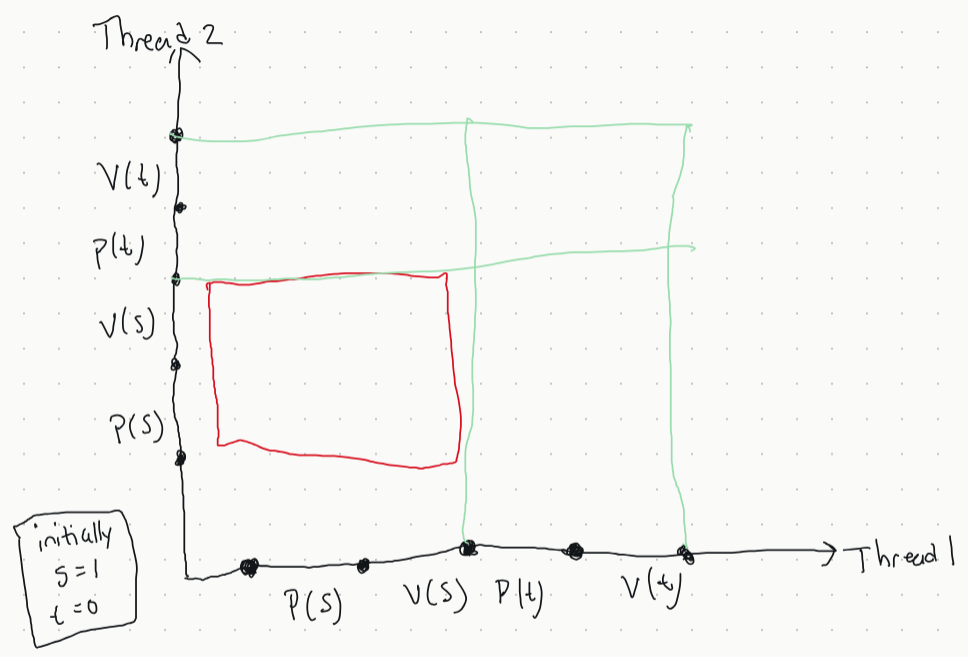
\includegraphics[width=0.75\textwidth]{exercise-12-15-progress-graph-deadlock}
			\caption{Exercise 12.15(a): Progress graph}
			\label{fig:ex-12-15a}
		\end{figure}
		\item The program always deadlocks because $t=0$.
		\item We can change $t$ to be 1 initially instead of 0.
		\item The updated deadlock-free progress graph is in Figure~\ref{fig:ex-12-15b}.
		\begin{figure}
			\centering
			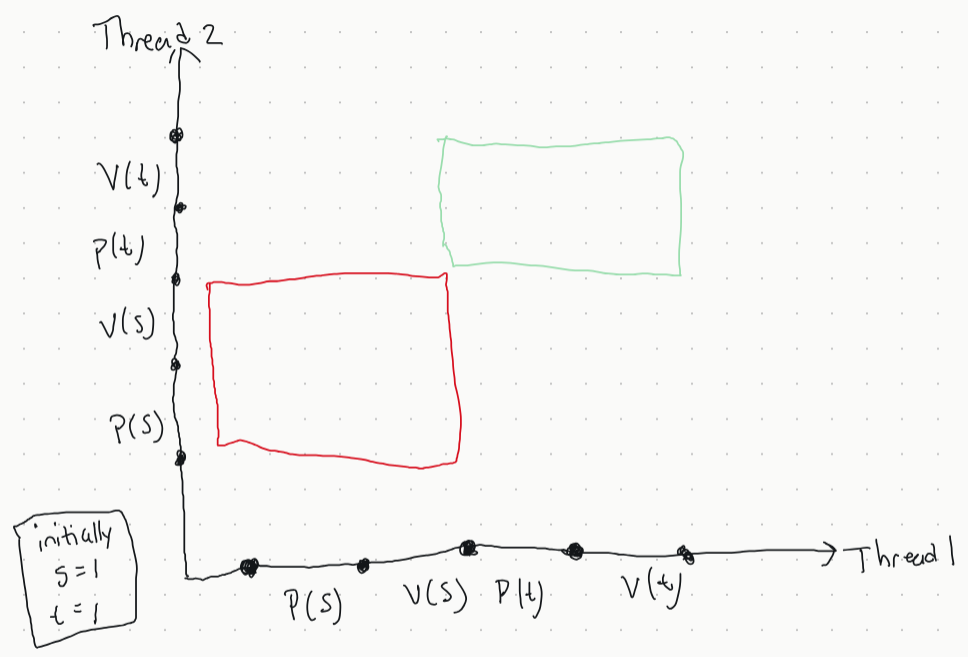
\includegraphics[width=0.75\textwidth]{exercise-12-15-progress-graph-deadlock-free}
			\caption{Exercise 12.15(a): Progress graph}
			\label{fig:ex-12-15b}
		\end{figure}
	\end{enumerate}
\end{sol}
\end{document}
